%\iffalse
\let\negmedspace\undefined
\let\negthickspace\undefined
\documentclass[journal,12pt,twocolumn]{IEEEtran}
\usepackage{cite}
\usepackage{amsmath,amssymb,amsfonts,amsthm}
\usepackage{algorithmic}
\usepackage{graphicx}
\usepackage{textcomp}
\usepackage{xcolor}
\usepackage{txfonts}
\usepackage{listings}
\usepackage{enumitem}
\usepackage{mathtools}
\usepackage{gensymb}
\usepackage{comment}
\usepackage[breaklinks=true]{hyperref}
\usepackage{tkz-euclide} 
\usepackage{listings}
\usepackage{gvv}                                        
\def\inputGnumericTable{}                                 
\usepackage[latin1]{inputenc}                                
\usepackage{color}                                            
\usepackage{array}                                            
\usepackage{longtable}                                       
\usepackage{calc}                                             
\usepackage{multirow}                                         
\usepackage{hhline}                                           
\usepackage{ifthen}                                           
\usepackage{lscape}
\newtheorem{theorem}{Theorem}[section]
\newtheorem{problem}{Problem}
\newtheorem{proposition}{Proposition}[section]
\newtheorem{lemma}{Lemma}[section]
\newtheorem{corollary}[theorem]{Corollary}
\newtheorem{example}{Example}[section]
\newtheorem{definition}[problem]{Definition}
\newcommand{\BEQA}{\begin{eqnarray}}
\newcommand{\EEQA}{\end{eqnarray}}
\newcommand{\define}{\stackrel{\triangle}{=}}
\theoremstyle{remark}
\newtheorem{rem}{Remark}
\begin{document}
\bibliographystyle{IEEEtran}
\vspace{3cm}
\title{NCERT: 11.9.3.2}
\author{EE23BTECH11040 - Manoj Kumar Ambatipudi$^{*}$% <-this % stops a space
}
\maketitle
\newpage
\bigskip
\renewcommand{\thefigure}{\theenumi}
\renewcommand{\thetable}{\theenumi}
\textbf{QUESTION:}
Find the $12^{th}$ term of a G.P. whose $8^{th}$ term is 192 and common ratio is 2.\\\\
\textbf{SOLUTION:}
\begin{table}[h!!]
\renewcommand\thetable{1}
    \centering
    \begin{tabular}{|c|c|c|}
    \hline
        Variable&             Description&value\\\hline
             $r$&            common ratio&2    \\\hline
     $x\brak{7}$&              eighth term&192  \\\hline
    \end{tabular}
    \caption{Variables Used and their Descriptions}
    \label{tab 11.9.3.2.1}
\end{table}


General term can be written as 
\begin{align}
    x\brak{n}=x\brak{0}r^{n}u\brak{n}\label{11.9.3.2.1}
\end{align}
Now on Z-transforming, we get
\begin{align}
    X\brak{z}=\frac{x\brak{0}}{1-rz^{-1}}\label{11.9.3.2.2} \quad   \abs{z}>\abs{r}
\end{align}
Referring to \tabref{tab 11.9.3.2.1}
\begin{align}
         x\brak{7}&=192\\
\implies x\brak{0}2^{7}&=192\\
\implies x\brak{0}&=\frac{3}{2}
\end{align}
The general term is written as \eqref{11.9.3.2.1}
\begin{align}
    x\brak{n}=\frac{3}{2}\times2^{n}u(n)
\end{align}
From \eqref{11.9.3.2.2} and \tabref{tab 11.9.3.2.1}, we get
\begin{align}
   \boxed{X\brak{z}=\frac{3}{1-2z^{-1}}}\quad   \abs{z}>2
\end{align}
From \tabref{tab 11.9.3.2.1} 
\begin{align}
x\brak{11} = 1.5\times2^{11} = 3072
\end{align}
\begin{figure}[h]
\renewcommand\thefigure{1} 
    \centering
    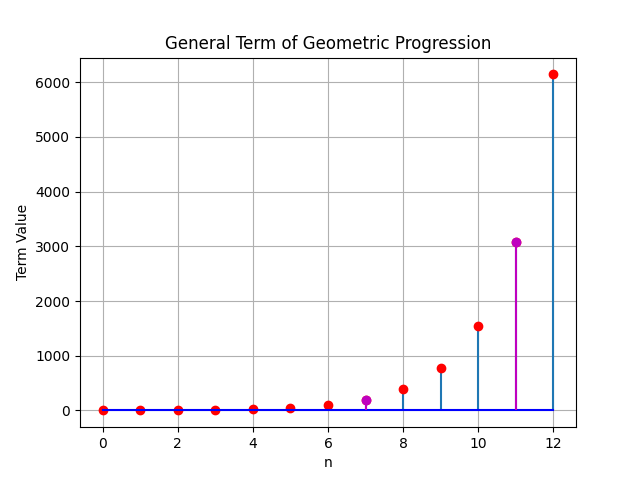
\includegraphics[width=1.0\columnwidth]{Fig_3.png}
    \caption{Plot of the general term taken from Python3}
    \label{fig:1}
\end{figure}
\end{document}
